\documentclass[../labs.tex]{subfiles}

\pagestyle{main}
\renewcommand{\leftmark}{Lab Report \thesection}
\setcounter{section}{3}

\begin{document}




\noindent Steven Labalme\\
2 February 2023\hfill
16 February 2023

\section{NMR ANALYSIS OF HEXYLAMINE}
\begin{figure}[H]
    \centering
    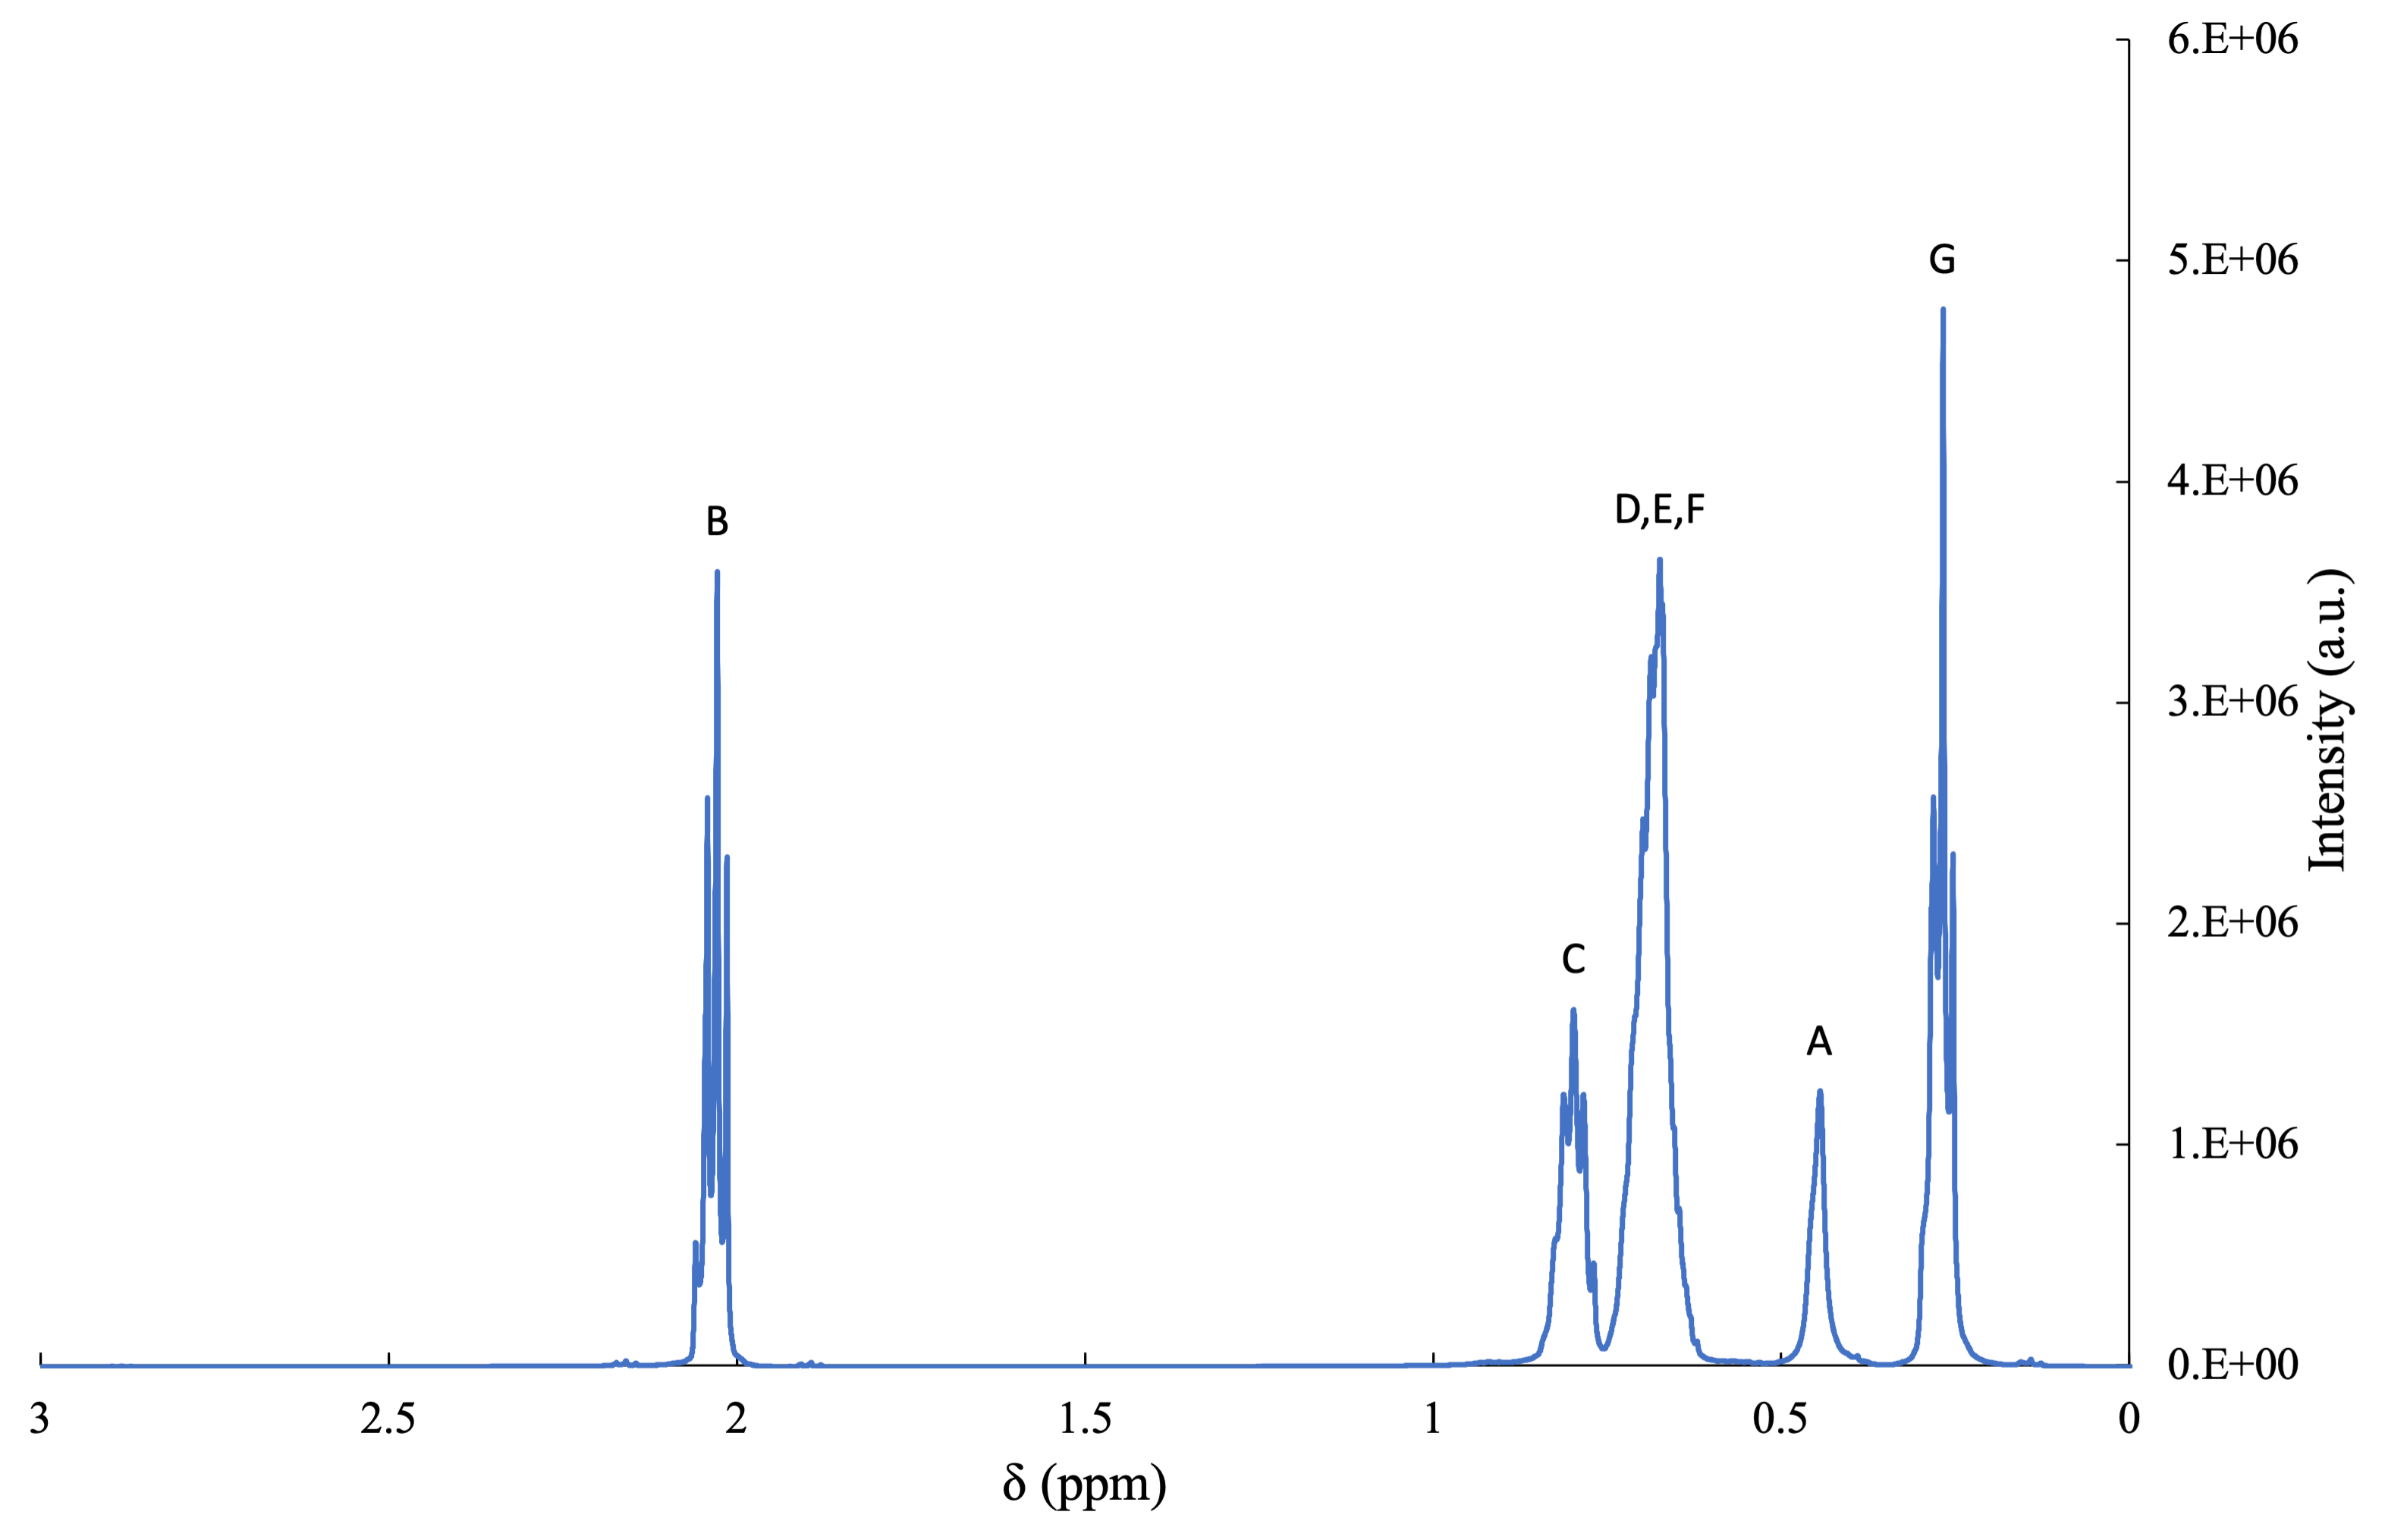
\includegraphics[width=0.95\linewidth]{hexylamineH1.png}
    \begin{tikzpicture}[remember picture,overlay,xshift=-12cm,yshift=8cm]
        \footnotesize
        \node{
            \chemfig{@{HG}-[:30]@{HF}-[:-30]@{HE}-[:30]@{HD}-[:-30]@{HC}-[:30]@{HB}-[:-30]N@{HA}H_2}
            \chemmove{
                \node [above=4pt] at (HA) {A};
                \node [above] at (HB) {B};
                \node [below] at (HC) {C};
                \node [above] at (HD) {D};
                \node [below] at (HE) {E};
                \node [above] at (HF) {F};
                \node [below] at (HG) {G};
            }
        };
    \end{tikzpicture}
    \caption{\ce{{}^1H} NMR spectrum of hexylamine. The protons on nitrogen exchange rapidly in solution, so since chemical exchanges cause spin decoupling, the A peak is a singlet.}
    \label{fig:hexylamineH1}
\end{figure}

\begin{figure}[H]
    \centering
    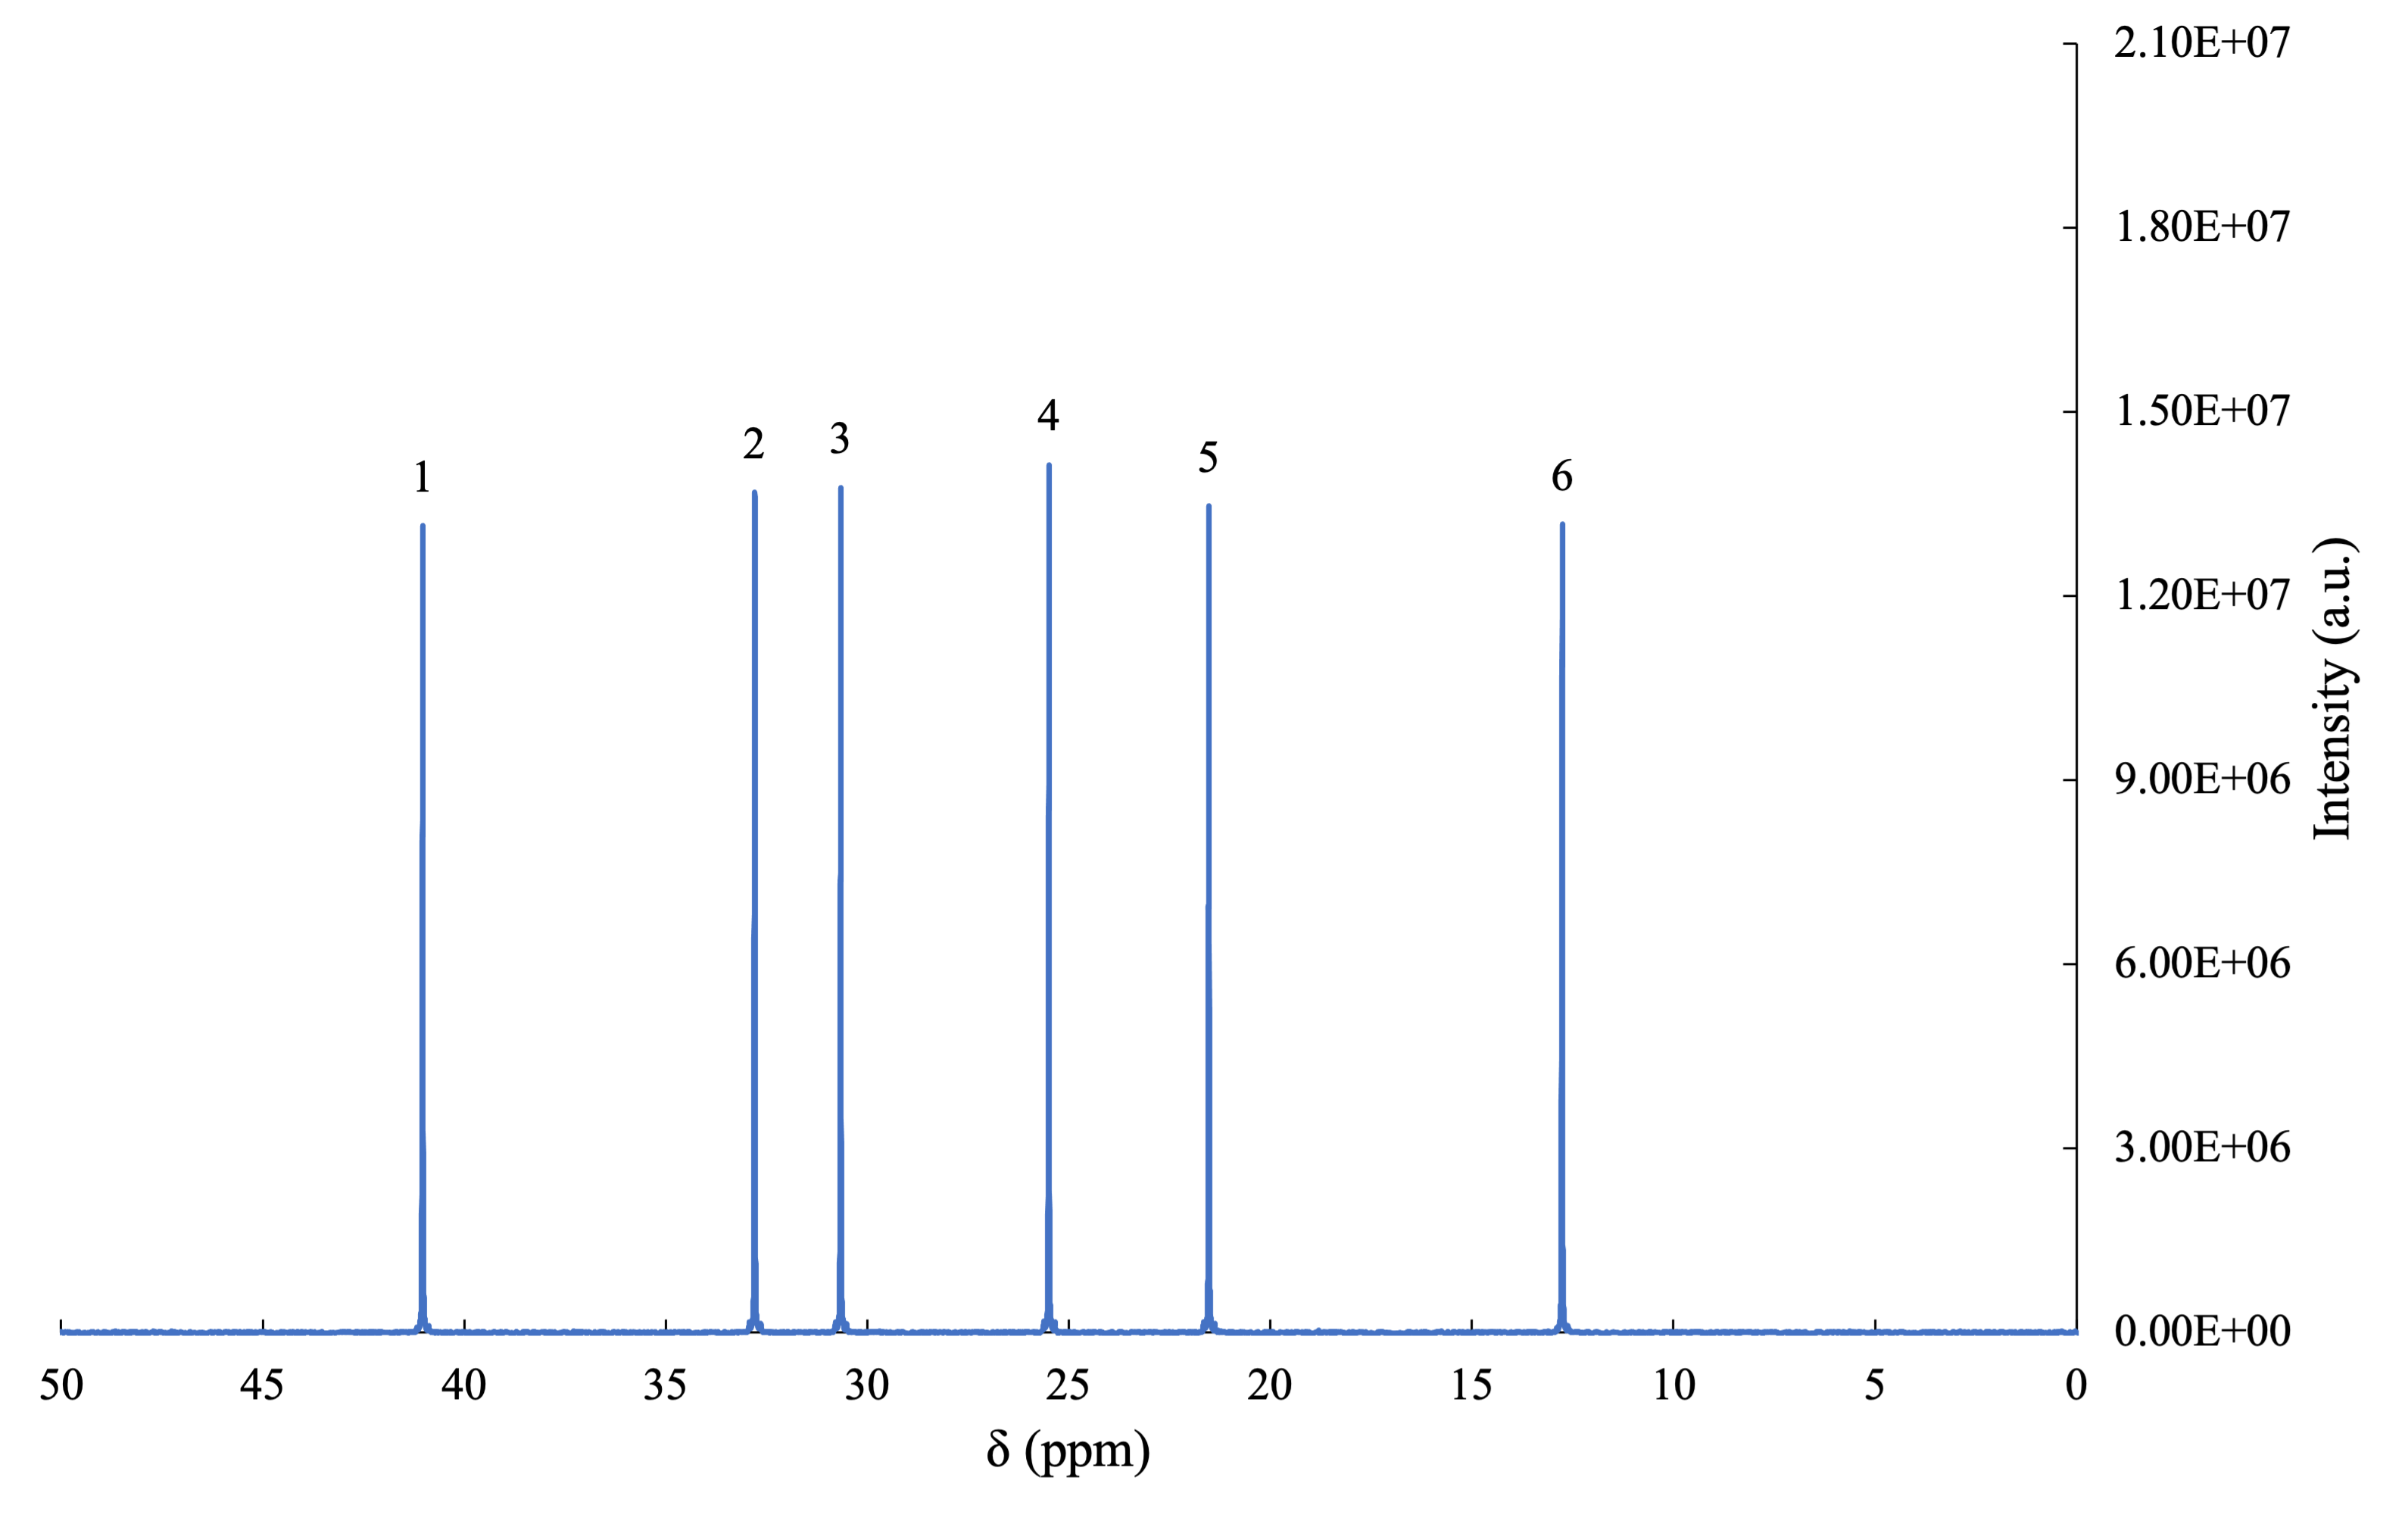
\includegraphics[width=0.95\linewidth]{hexylamineC13.png}
    \begin{tikzpicture}[remember picture,overlay,xshift=-12cm,yshift=8.5cm]
        \footnotesize
        \node{
            \chemfig{@{C6}-[:30]@{C5}-[:-30]@{C4}-[:30]@{C3}-[:-30]@{C2}-[:30]@{C1}-[:-30]NH_2}
            \chemmove{
                \node [above] at (C1) {1};
                \node [below] at (C2) {2};
                \node [above] at (C3) {3};
                \node [below] at (C4) {4};
                \node [above] at (C5) {5};
                \node [below] at (C6) {6};
            }
        };
    \end{tikzpicture}
    \caption{\ce{{}^13C} NMR spectrum of hexylamine. Notice that carbon 1 is the most downshifted because it's closest to the electronegative nitrogen atom.}
    \label{fig:hexylamineC13}
\end{figure}

\begin{figure}[H]
    \centering
    \begin{subfigure}[b]{0.49\linewidth}
        \centering
        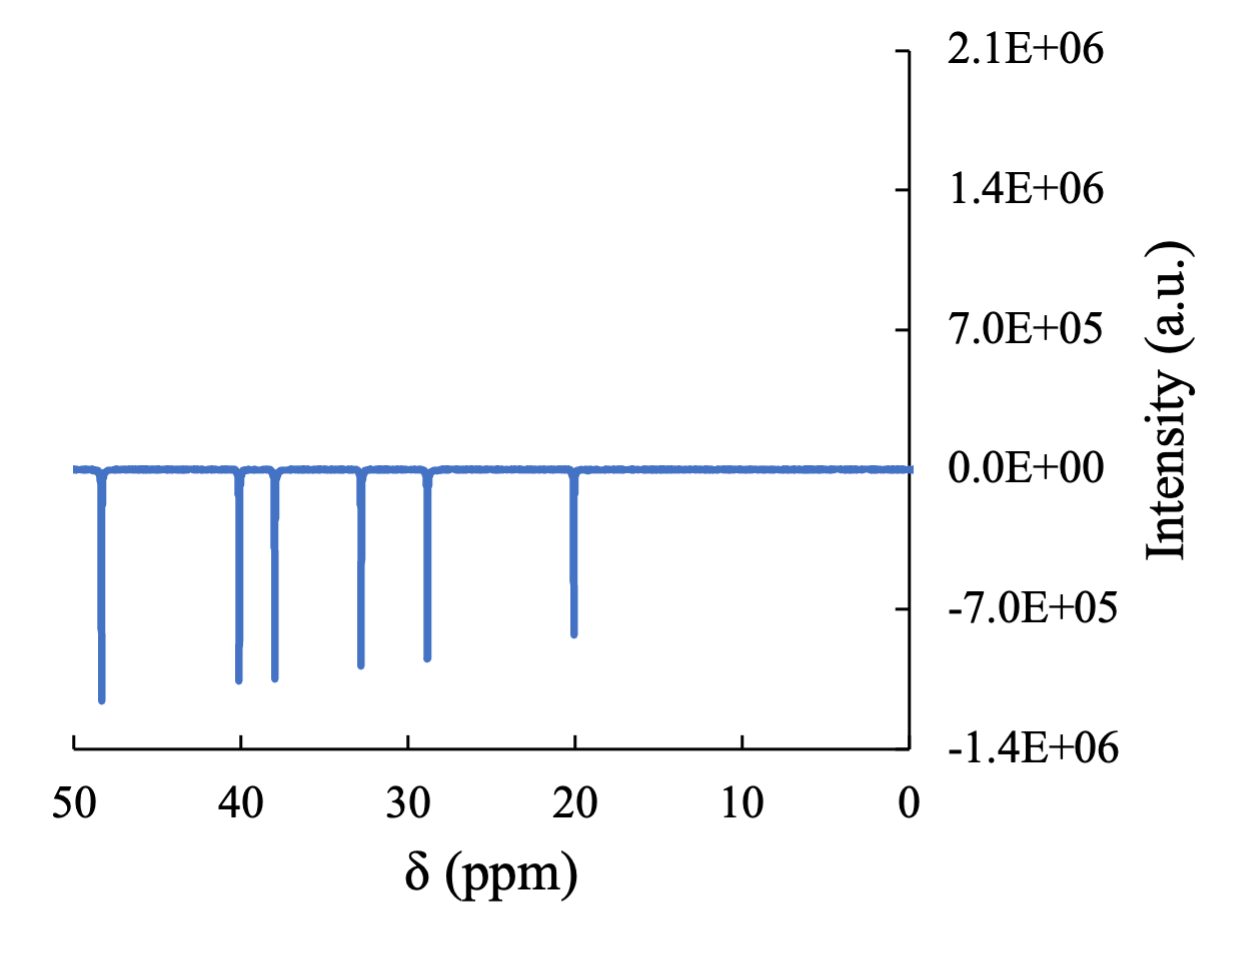
\includegraphics[width=0.9\linewidth]{C13repa.png}
        \caption{$\tau=\SI{0.001}{\second}$.}
        \label{fig:C13repa}
    \end{subfigure}
    \begin{subfigure}[b]{0.49\linewidth}
        \centering
        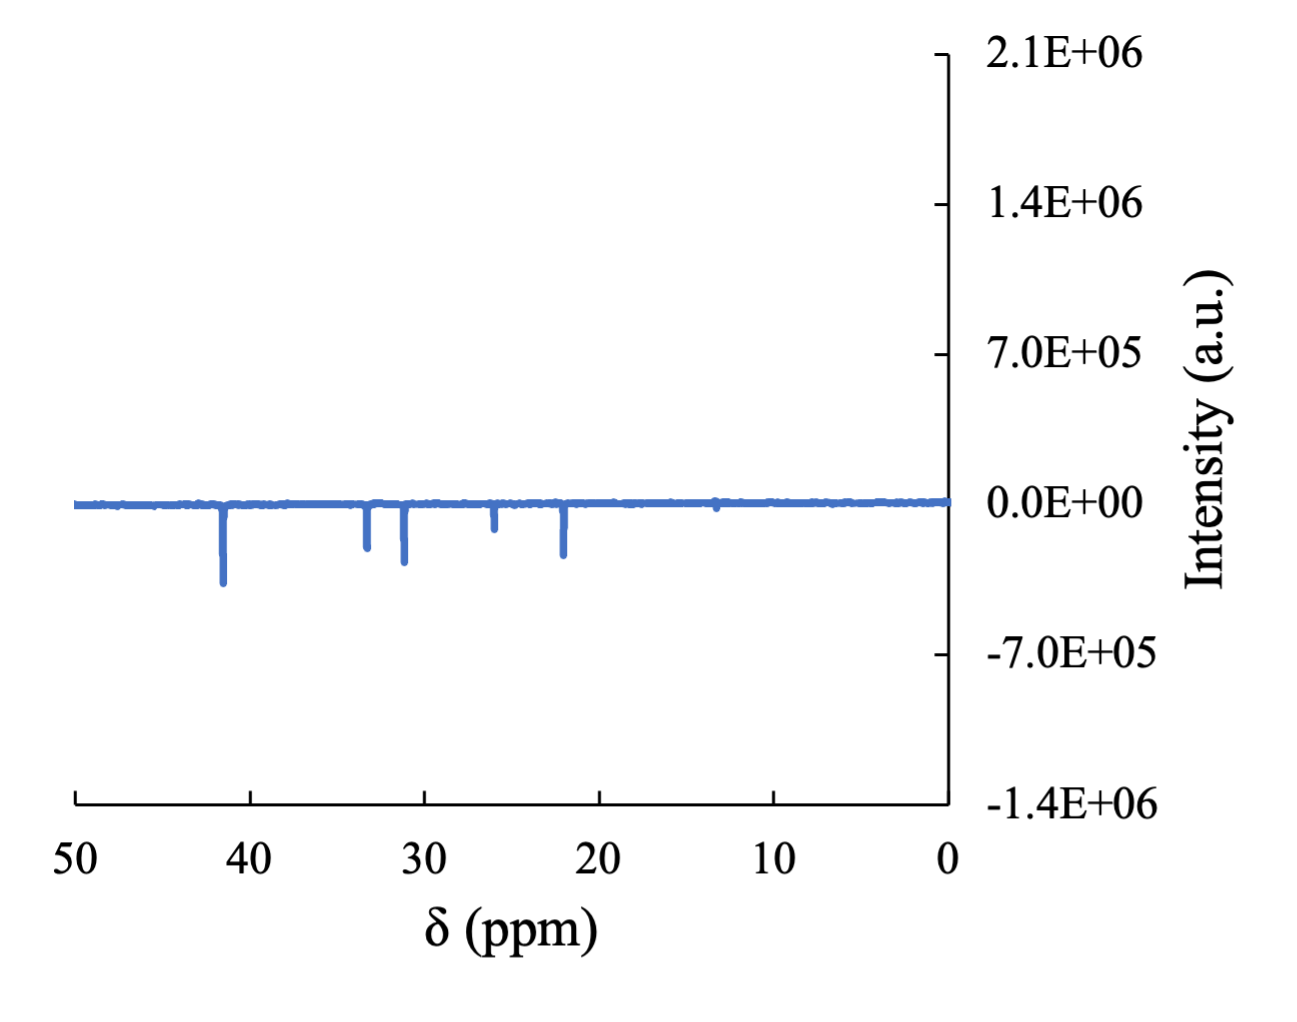
\includegraphics[width=0.9\linewidth]{C13repb.png}
        \caption{$\tau=\SI{2.5}{\second}$.}
        \label{fig:C13repb}
    \end{subfigure}\\[1em]
    \begin{subfigure}[b]{0.49\linewidth}
        \centering
        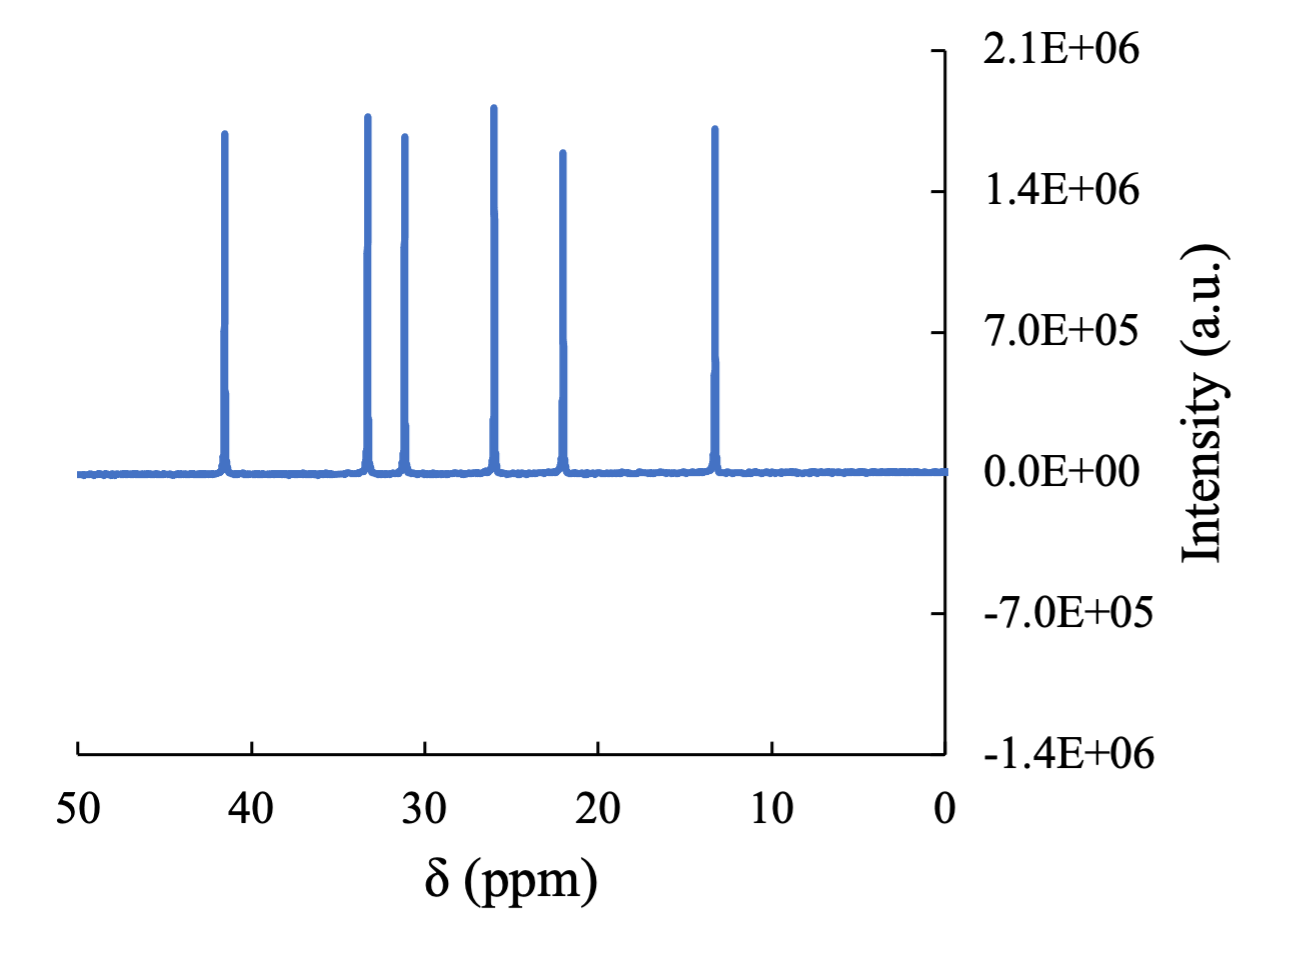
\includegraphics[width=0.9\linewidth]{C13repc.png}
        \caption{$\tau=\SI{10}{\second}$.}
        \label{fig:C13repc}
    \end{subfigure}
    \caption{A selection of inversion recovery \ce{{}^13C} NMR spectra for different delay times $\tau$.}
    \label{fig:C13rep}
\end{figure}

\begin{figure}[H]
    \centering
    \begin{subfigure}[b]{0.49\linewidth}
        \centering
        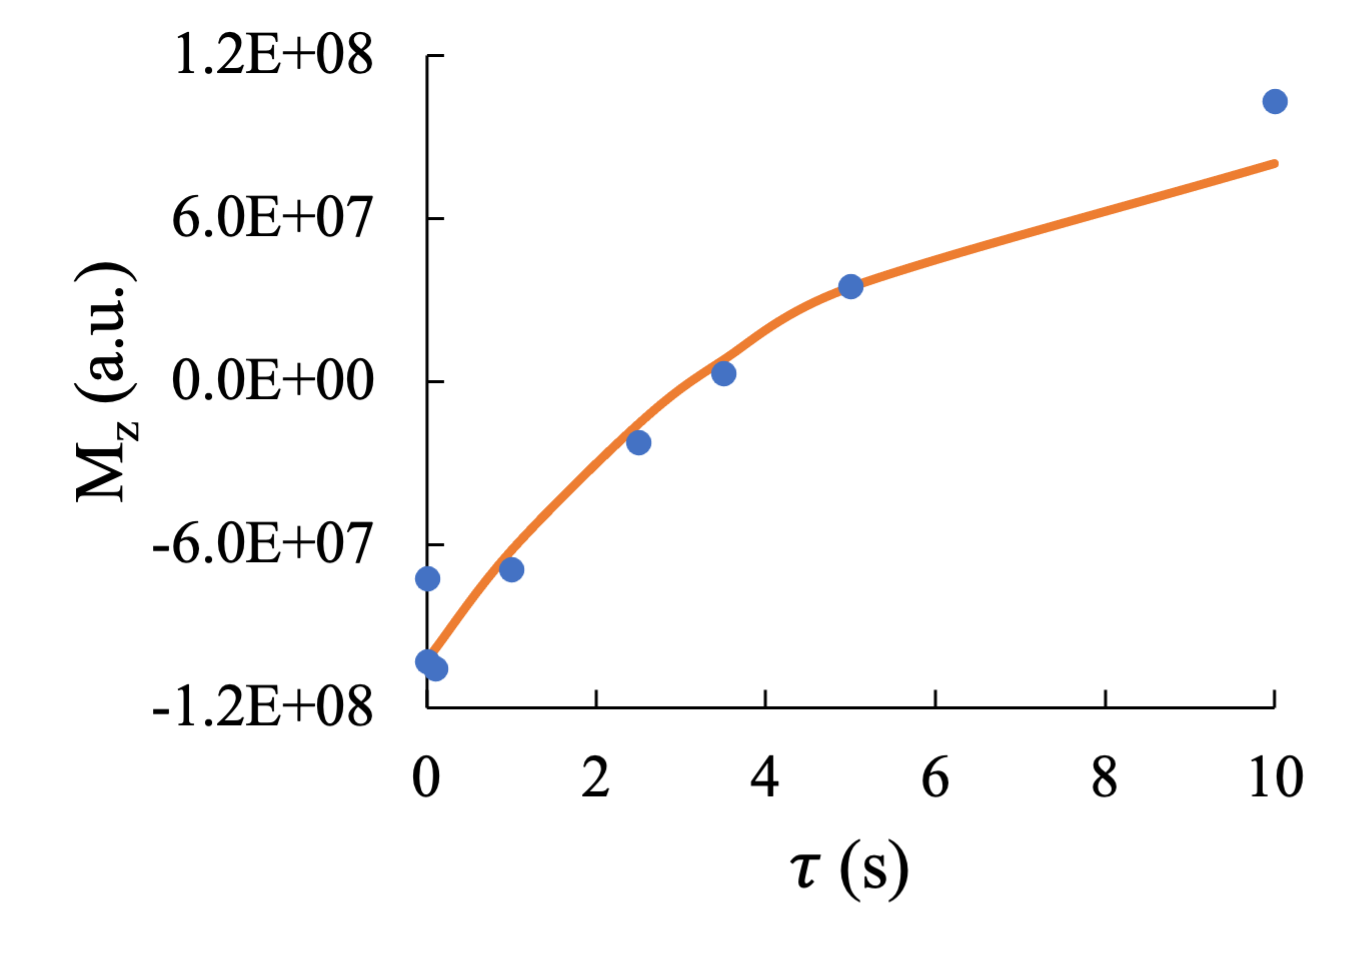
\includegraphics[width=0.9\linewidth]{T1M0a.png}
        \caption{Carbon 1.}
        \label{fig:T1M0a}
    \end{subfigure}
    \begin{subfigure}[b]{0.49\linewidth}
        \centering
        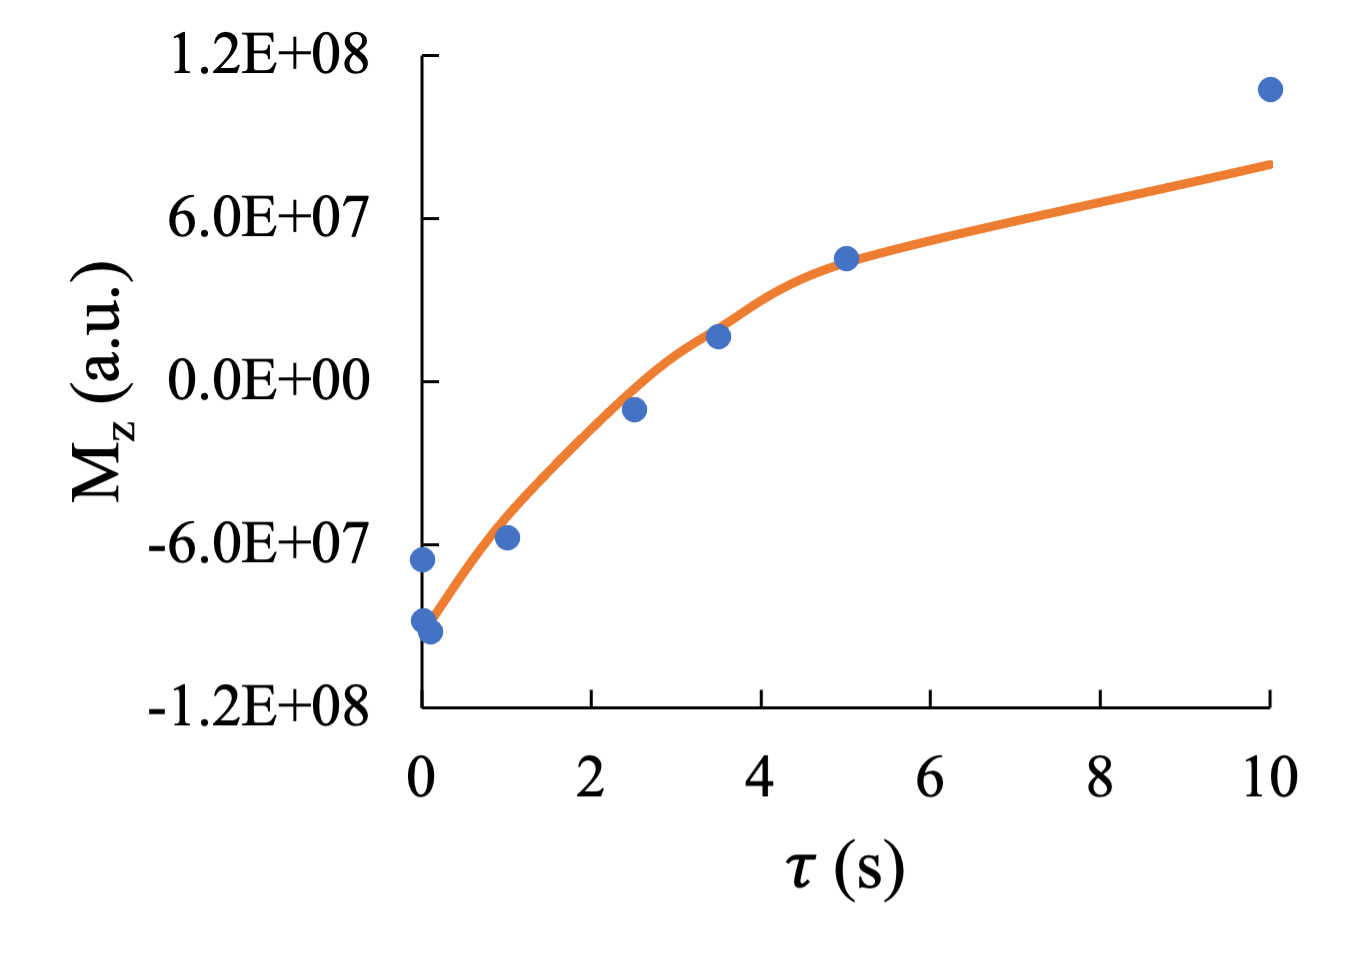
\includegraphics[width=0.9\linewidth]{T1M0b.png}
        \caption{Carbon 2.}
        \label{fig:T1M0b}
    \end{subfigure}\\[1em]
    \begin{subfigure}[b]{0.49\linewidth}
        \centering
        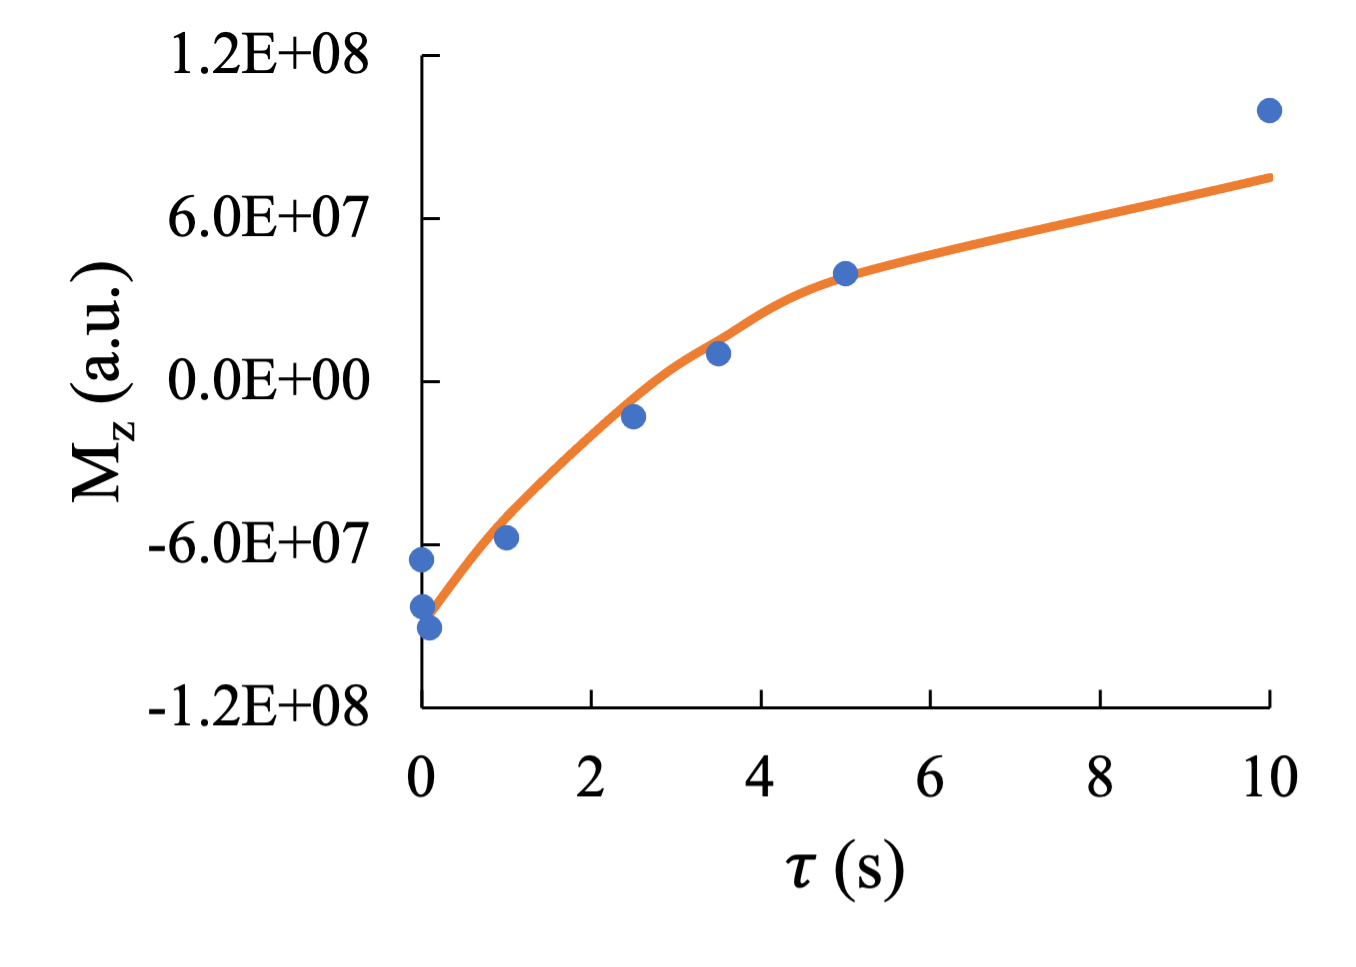
\includegraphics[width=0.9\linewidth]{T1M0c.png}
        \caption{Carbon 3.}
        \label{fig:T1M0c}
    \end{subfigure}
    \begin{subfigure}[b]{0.49\linewidth}
        \centering
        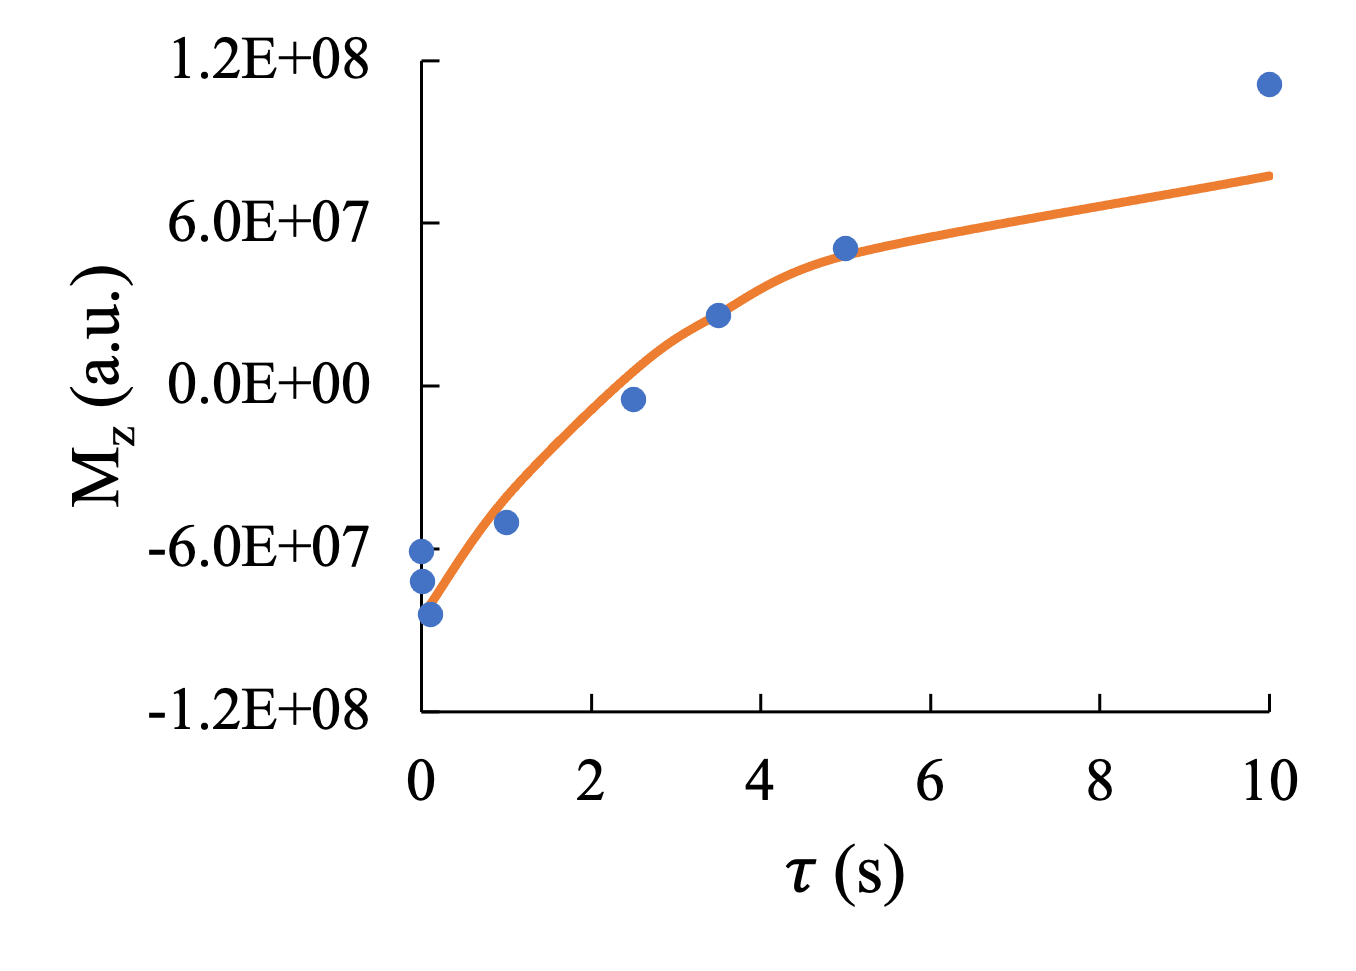
\includegraphics[width=0.9\linewidth]{T1M0d.png}
        \caption{Carbon 4.}
        \label{fig:T1M0d}
    \end{subfigure}\\[1em]
    \begin{subfigure}[b]{0.49\linewidth}
        \centering
        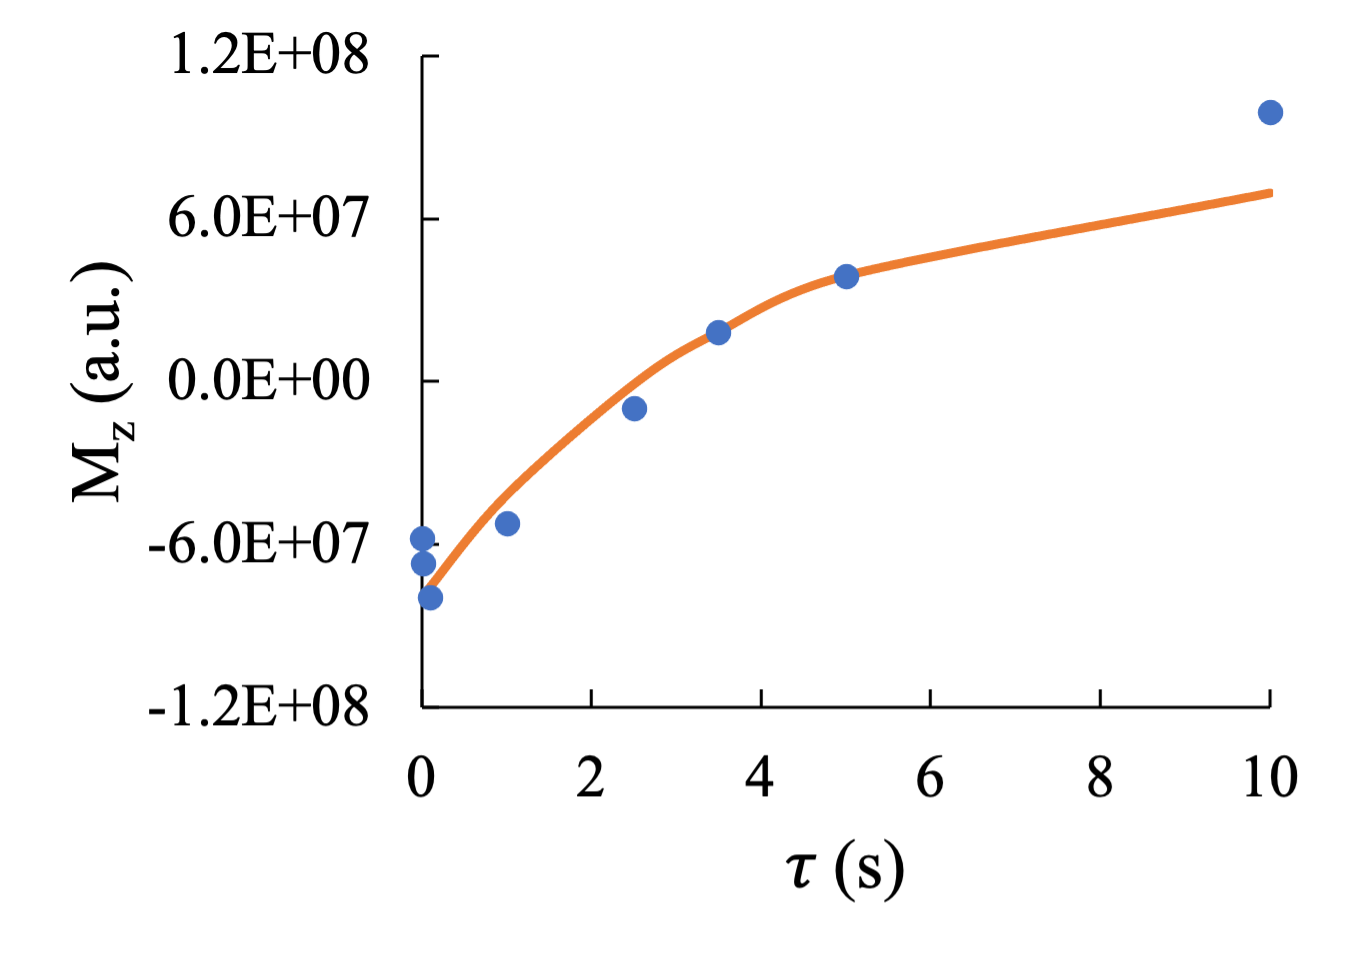
\includegraphics[width=0.9\linewidth]{T1M0e.png}
        \caption{Carbon 5.}
        \label{fig:T1M0e}
    \end{subfigure}
    \begin{subfigure}[b]{0.49\linewidth}
        \centering
        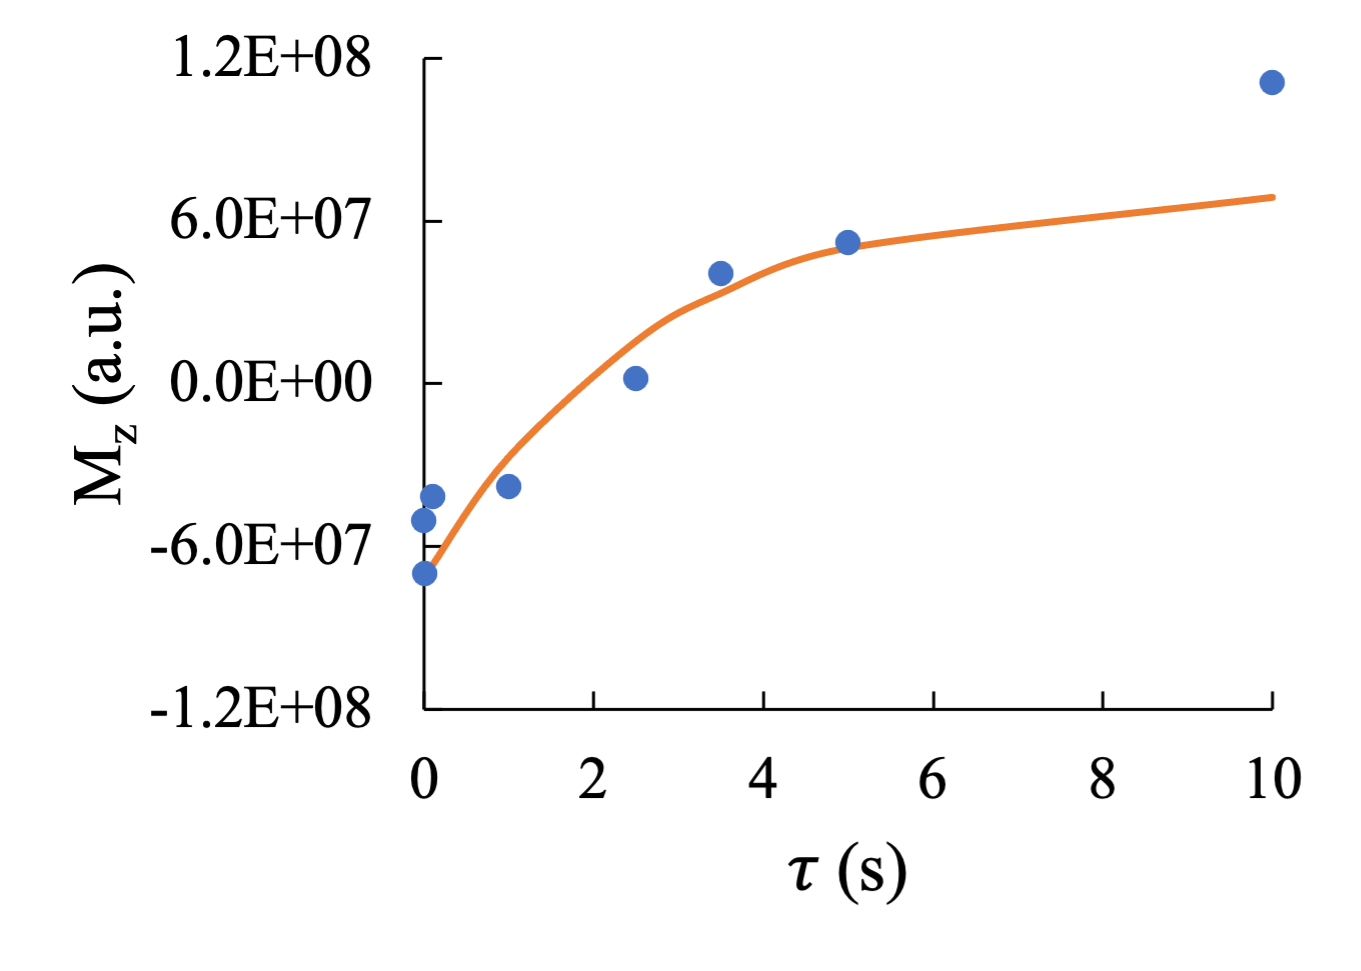
\includegraphics[width=0.9\linewidth]{T1M0f.png}
        \caption{Carbon 6.}
        \label{fig:T1M0f}
    \end{subfigure}
    \caption{Determining the spin-lattice relaxation time $T_1$ and the magnetization $M_0$ at equilibrium via nonlinear regression.}
    \label{fig:T1M0}
\end{figure}

\begin{table}[H]
    \centering
    \small
    \renewcommand{\arraystretch}{1.2}
    \begin{tabular}{|c|c|c|c|c|c|}
        \hline
        \textbf{Carbon 1} & \textbf{Carbon 2} & \textbf{Carbon 3} & \textbf{Carbon 4} & \textbf{Carbon 5} & \textbf{Carbon 6}\\
        \hline
        \num{15197494.17} & \num{15490978.25} & \num{14146608.68} & \num{17608862.89} & \num{15739108.37} & \num{21625158.79}\\
        \hline
    \end{tabular}
    \caption{Standard errors for the above nonlinear regressions.}
    \label{fig:NMRse}
\end{table}

\begin{table}[H]
    \centering
    \small
    \renewcommand{\arraystretch}{1.2}
    \begin{tabular}{|c|c|c|c|c|c|c|}
        \hline
         & \textbf{Carbon 1} & \textbf{Carbon 2} & \textbf{Carbon 3} & \textbf{Carbon 4} & \textbf{Carbon 5} & \textbf{Carbon 6}\\
        \hline
        \textbf{$\bm{T_1}$ (s)} & \num{4.52} & \num{3.75} & \num{3.99} & \num{3.29} & \num{3.67} & \num{2.66}\\ \hline
        \textbf{$\bm{\tau_C^{}}$ (ps/rad)} & \num{5.15} & \num{6.21} & \num{5.83} & \num{7.07} & \num{6.34} & \num{5.83}\\
        \hline
    \end{tabular}
    \caption{The spin-lattice relaxation time and correlation time for each carbon in hexylamine.}
    \label{tab:T1tC}
\end{table}
Note that to calculate $\tau_C$ from $T_1$, the formula
\begin{equation*}
    \frac{1}{T_1} = n\left( \frac{\mu_0}{4\pi} \right)^2\frac{\hbar^2\gamma_{\ce{C}}^2\gamma_{\ce{H}}^2}{r_{\ce{CH}}^6}\tau_{\ce{C}}
\end{equation*}
was used, where the values of $\gamma_{\ce{C}}$ and $\gamma_{\ce{H}}$ were obtained from \textcite{bib:C13H1gyro} and the value of $r_{\ce{CH}}$ was obtained from \textcite{bib:CRCHandbook}.\par\medskip
% $T_1$ is the time constant governing the restoration of equilibrium to $M_z$ after being disturbed away by a pulse. The $T_1$ values generally trend down. $T_1$ depends on intramolecular interactions and on a molecular motion. We'll say that the motion of the polar end is restricted by hydrogen bonding. $\tau_C$ is about freedom of movement, too.
$T_1$ is the time constant governing how quickly magnetic spins return to equilibrium after a disturbance. The data in Table \ref{tab:T1tC} shows that $T_1$ trends downward for carbon atoms progressively farther from the amine moiety. This implies that carbons farther from the \ce{NH2} group return to equilibrium more quickly. This would support a theory that the hydrogen-bonding interactions present at the \ce{NH2} group restrict freedom in this molecule, and that portions of it farther from the center of restriction can move more freely and equilibrate more quickly. Since $\tau_C$ is related to freedom of motion directly (it is literally a measure of the time required to change angle), the above commentary also applies to it.

\begin{figure}[h!]
    \centering
    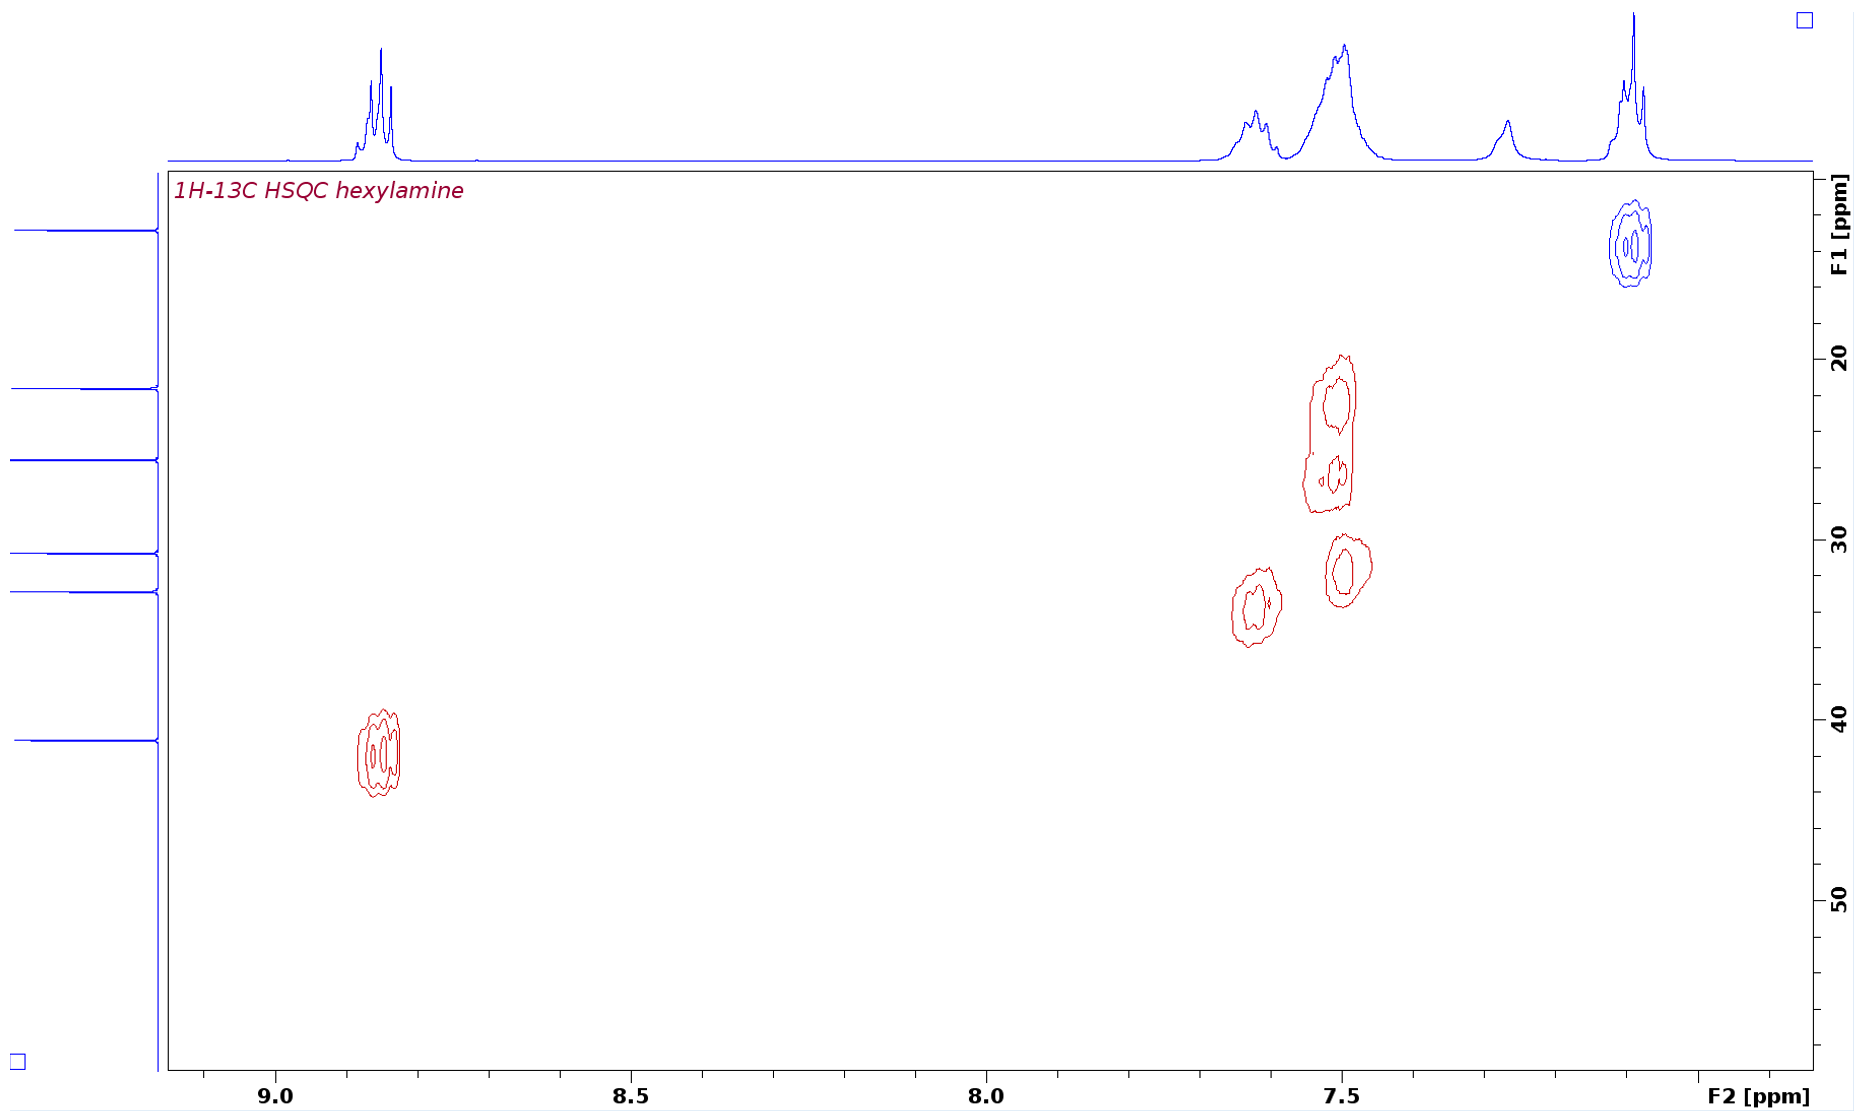
\includegraphics[width=0.9\linewidth]{1H13CHSQC.png}
    \caption{Two-dimensional \ce{{}^1H}-\ce{{}^13C} HSQC spectrum of hexylamine.}
    \label{fig:1H13CHSQC}
\end{figure}
The peaks at the top of the HSQC spectrum in Figure \ref{fig:1H13CHSQC} are analogous to those in the \ce{{}^1H} spectrum of hexylamine. Similarly, those on the left side of the above image are analogous to those in the \ce{{}^13C} spectrum of hexylamine. HSQC transfers magnetism between bound protons and \ce{{}^13C} atoms atoms, so moieties that resonate in both forms of spectroscopy show up as two-dimensional peaks; in other words, each 2D peak corresponds to the proton above it and the carbon to the left of it. Thus, the six distinct peaks in the 2D spectrum correspond to the six carbons and their associated protons. The one hydrogen peak with no corresponding carbon peak represents the protons on the \ce{NH2} moiety, providing additional evidence for the identification of that peak beyond the fact that it's a singlet per rapid proton transfer-induced spin decoupling.
\newpage


\printbibliography
\setcounter{figure}{0}
\setcounter{table}{0}




\end{document}